\documentclass{ximera}
\title{Polynomial and Rational Inequalities}

\outcome{Solve polynomial inequalities using sign analysis.}
\outcome{Solve rational inequalities by isolating zero and using sign analysis.}
\outcome{Read the solution to an inequality from a graph.}
\outcome{Find the domain of a function involving a square root using inequality techniques.}

\begin{document}
\begin{abstract}
\end{abstract}
\maketitle

\textbf{Learning Objectives:}
\begin{itemize}
  \item Solve polynomial and rational inequalities using sign analysis.
  \item Always isolate 0 first; never multiply across an inequality by a variable expression.
  \item Read solutions to inequalities directly from a graph.
  \item Find the domain of a radical function using inequality techniques.
\end{itemize}
\medskip

\noindent\textbf{Key Strategy:} Move everything to one side (isolate 0), factor completely, identify boundary points, then test signs on each interval.

\bigskip
\section*{Quick Check}

\begin{problem}
Solve: $x^2+3x > 10$.
\begin{hint}
Isolate 0: $x^2+3x-10 > 0$. Factor, find boundary points, then test signs.
\end{hint}
\begin{multipleChoice}
  \choice{$(-\infty,0)\cup(3,\infty)$}
  \choice{$(-2,5)$}
  \choice[correct]{$(-\infty,-5)\cup(2,\infty)$}
  \choice{$(0,3)$}
  \choice{Not listed}
\end{multipleChoice}
\end{problem}

\begin{problem}
Solve: $\ds\dfrac{(x-3)(x+1)}{-2x^2}\geq 0$.
\begin{hint}
The denominator $-2x^2 \leq 0$ for all $x$ (equals zero at $x=0$). For the fraction to be $\geq 0$, the numerator must also be $\leq 0$. Solve $(x-3)(x+1)\leq 0$ and exclude $x=0$.
\end{hint}
\begin{multipleChoice}
  \choice{$[-1,3]$}
  \choice{$(-\infty,-1]\cup[3,\infty)$}
  \choice{$(-\infty,-1)\cup(0,3]$}
  \choice[correct]{$[-1,0)\cup(0,3]$}
  \choice{Not listed}
\end{multipleChoice}
\end{problem}

\begin{problem}
Which expression is equivalent to $\ds\dfrac{3-x}{x+2}\geq 4$?
\begin{hint}
Subtract 4 from both sides, find a common denominator, and combine into a single fraction.
\end{hint}
\begin{multipleChoice}
  \choice{$3-x\leq 4(x+2)$}
  \choice{$\dfrac{x+1}{x+2}\geq 0$}
  \choice[correct]{$\dfrac{-5(x+1)}{x+2}\geq 0$}
  \choice{$4\geq\dfrac{3-x}{x+2}$}
  \choice{$x\geq -1$}
\end{multipleChoice}
\end{problem}

\begin{problem}
Express the domain of $f(x)=\sqrt{2x-x^2}$ in interval notation.
\begin{hint}
You need $2x-x^2 \geq 0$. Factor: $x(2-x) \geq 0$.
\end{hint}
\begin{multipleChoice}
  \choice{$[0,\infty)$}
  \choice[correct]{$[0,2]$}
  \choice{$(0,2)$}
  \choice{$(-\infty,0]\cup[2,\infty)$}
  \choice{Not listed}
\end{multipleChoice}
\end{problem}

\begin{problem}
Which inequality has solution set $(-\infty,-3]\cup[1,\infty)$?
\begin{hint}
Factor each option and identify which gives zeros at $x=-3$ and $x=1$ with the correct inequality direction.
\end{hint}
\begin{multipleChoice}
  \choice{$x^2+2x-3\leq 0$}
  \choice[correct]{$x^2+2x-3\geq 0$}
  \choice{$x^2-2x-3\leq 0$}
  \choice{$(x+3)(x-1)<0$}
  \choice{Not listed}
\end{multipleChoice}
\end{problem}


\bigskip
\section*{Extended Practice}

\begin{problem}
Use the graphs of $f(x)$ below (Figures 1 and 2). Solve each inequality and write your answer in interval notation.

\begin{center}
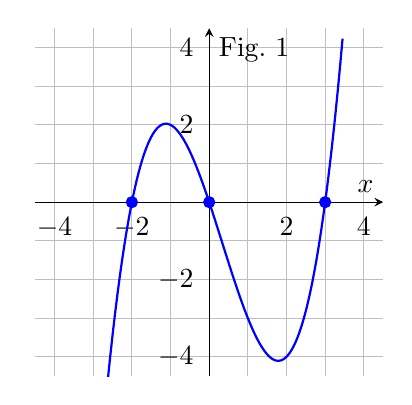
\begin{tikzpicture}
\begin{axis}[
  axis lines=center, width=6cm, height=6cm,
  xlabel={$x$}, ylabel={Fig.\ 1},
  xmin=-4.5, xmax=4.5, xtick={-4,-2,0,2,4},
  ymin=-4.5, ymax=4.5, ytick={-4,-2,0,2,4},
  grid=both, minor tick num=1, tick style={draw=none},
]
\addplot[thick, blue, domain=-2.62:3.45, samples=100] {0.5*x*(x+2)*(x-3)};
\addplot[only marks, mark=*, blue] coordinates {(0,0) (-2,0) (3,0)};
\end{axis}
\end{tikzpicture}
\qquad
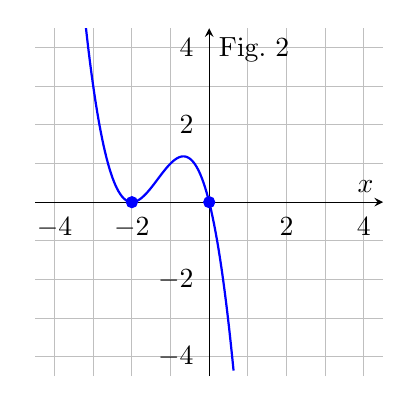
\begin{tikzpicture}
\begin{axis}[
  axis lines=center, width=6cm, height=6cm,
  xlabel={$x$}, ylabel={Fig.\ 2},
  xmin=-4.5, xmax=4.5, xtick={-4,-2,0,2,4},
  ymin=-4.5, ymax=4.5, ytick={-4,-2,0,2,4},
  grid=both, minor tick num=1, tick style={draw=none},
]
\addplot[thick, blue, domain=-3.2:0.63, samples=100] {-x*(x+2)^2};
\addplot[only marks, mark=*, blue] coordinates {(0,0) (-2,0)};
\end{axis}
\end{tikzpicture}
\end{center}

\medskip
\textbf{(a)} Figure 1 (polynomial with zeros at $x=-2$, $x=0$, $x=3$):
\begin{enumerate}
  \item[(i)] $f(x) > 0$
  \item[(ii)] $f(x) \leq 0$
  \item[(iii)] $f(x) < 0$
\end{enumerate}

\medskip
\textbf{(b)} Figure 2 (function with even-multiplicity zero at $x=-2$ and zero at $x=0$):
\begin{enumerate}
  \item[(i)] $f(x) \leq 0$
  \item[(ii)] $f(x) > 0$
  \item[(iii)] $f(x) \geq 0$
\end{enumerate}

\begin{solution}
\textbf{(a)} Sign of $f(x)$:
\begin{center}
\begin{tikzpicture}
\begin{axis}[
  axis y line=none, axis lines=left, axis line style={latex-latex},
  xmin=-3.9, xmax=4.9, ymin=0, ymax=1, xlabel=$x$,
  scatter/classes={a={mark=*,red,mark size=2pt},b={mark=x,draw=red,mark size=4pt}},
  restrict y to domain=0:1, xtick={-2,0,3}]
\addplot[<->,scatter,only marks,scatter src=explicit symbolic]
  table [y expr=0,meta index=1,header=false] {
  -2 a
  0 a
  3 a
  };
\node[coordinate,label=above:{$-$}] at (axis cs:-2.9,0.05) {};
\node[coordinate,label=above:{$+$}] at (axis cs:-1,0.05) {};
\node[coordinate,label=above:{$-$}] at (axis cs:1.5,0.05) {};
\node[coordinate,label=above:{$+$}] at (axis cs:3.9,0.05) {};
\end{axis}
\end{tikzpicture}
\end{center}
\begin{enumerate}
  \item[(i)] $f(x) > 0$: $(-2,0)\cup(3,\infty)$
  \item[(ii)] $f(x) \leq 0$: $(-\infty,-2]\cup[0,3]$
  \item[(iii)] $f(x) < 0$: $(-\infty,-2)\cup(0,3)$
\end{enumerate}

\textbf{(b)} Sign of $f(x)$:
\begin{center}
\begin{tikzpicture}
\begin{axis}[
  axis y line=none, axis lines=left, axis line style={latex-latex},
  xmin=-3.9, xmax=1.9, ymin=0, ymax=1, xlabel=$x$,
  scatter/classes={a={mark=*,red,mark size=2pt},b={mark=x,draw=red,mark size=4pt}},
  restrict y to domain=0:1, xtick={-2,0}]
\addplot[<->,scatter,only marks,scatter src=explicit symbolic]
  table [y expr=0,meta index=1,header=false] {
  -2 a
  0 a
  };
\node[coordinate,label=above:{$+$}] at (axis cs:-2.9,0.05) {};
\node[coordinate,label=above:{$+$}] at (axis cs:-1,0.05) {};
\node[coordinate,label=above:{$-$}] at (axis cs:0.9,0.05) {};
\end{axis}
\end{tikzpicture}
\end{center}
\begin{enumerate}
  \item[(i)] $f(x) \leq 0$: $\{-2\}\cup[0,\infty)$
  \item[(ii)] $f(x) > 0$: $(-\infty,-2)\cup(-2,0)$
  \item[(iii)] $f(x) \geq 0$: $(-\infty,0]$
\end{enumerate}
\end{solution}
\end{problem}


\begin{problem}
Use the graph of $f(x)$ below (rational function with vertical asymptotes at $x=-3$ and $x=1$, even-multiplicity zero at $x=-2$, and simple zero at $x=0$). Solve each inequality.

\begin{center}
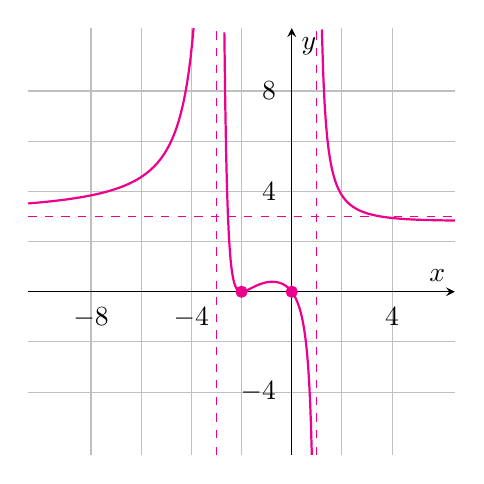
\begin{tikzpicture}
\begin{axis}[
  axis lines=center, width=7cm, height=7cm,
  xlabel={$x$}, ylabel={$y$},
  xmin=-10.5, xmax=6.5, xtick={-8,-4,0,4},
  ymin=-6.5, ymax=10.5, ytick={-4,0,4,8},
  grid=both, minor tick num=1, tick style={draw=none},
]
\addplot[thick, magenta, domain=-10.5:-3.9, samples=100] {(3*(x+2)^2*x)/((x+3)^2*(x-1))};
\addplot[thick, magenta, domain=-2.685:0.8, samples=100] {(3*(x+2)^2*x)/((x+3)^2*(x-1))};
\addplot[thick, magenta, domain=1.2:6.5, samples=100] {(3*(x+2)^2*x)/((x+3)^2*(x-1))};
\addplot[only marks, mark=*, magenta] coordinates {(-2,0) (0,0)};
\addplot[dashed, thin, magenta] coordinates {(-3,-6.5) (-3,10.5)};
\addplot[dashed, thin, magenta] coordinates {(1,-6.5) (1,10.5)};
\addplot[dashed, thin, magenta] coordinates {(-10.5,3) (6.5,3)};
\end{axis}
\end{tikzpicture}
\end{center}
\begin{enumerate}
  \item[(a)] $f(x) \geq 0$
  \item[(b)] $f(x) < 0$
  \item[(c)] $f(x) \leq 0$
  \item[(d)] $f(x) > 0$
\end{enumerate}

\begin{solution}
Sign of $f(x)$:
\begin{center}
\begin{tikzpicture}
\begin{axis}[
  axis y line=none, axis lines=left, axis line style={latex-latex},
  xmin=-3.9, xmax=1.9, ymin=0, ymax=1, xlabel=$x$,
  scatter/classes={a={mark=*,red,mark size=2pt},b={mark=x,draw=red,mark size=4pt}},
  restrict y to domain=0:1, xtick={-3,-2,0,1}]
\addplot[<->,scatter,only marks,scatter src=explicit symbolic]
  table [y expr=0,meta index=1,header=false] {
  -3 b
  -2 a
  0 a
  1 b
  };
\node[coordinate,label=above:{$+$}] at (axis cs:-3.4,0.05) {};
\node[coordinate,label=above:{$+$}] at (axis cs:-2.5,0.05) {};
\node[coordinate,label=above:{$+$}] at (axis cs:-1,0.05) {};
\node[coordinate,label=above:{$-$}] at (axis cs:0.5,0.05) {};
\node[coordinate,label=above:{$+$}] at (axis cs:1.4,0.05) {};
\end{axis}
\end{tikzpicture}
\end{center}
\begin{enumerate}
  \item[(a)] $f(x) \geq 0$: $(-\infty,-3)\cup(-3,0]\cup(1,\infty)$
  \item[(b)] $f(x) < 0$: $(0,1)$
  \item[(c)] $f(x) \leq 0$: $\{-2\}\cup[0,1)$
  \item[(d)] $f(x) > 0$: $(-\infty,-3)\cup(-3,-2)\cup(-2,0)\cup(1,\infty)$
\end{enumerate}
\end{solution}
\end{problem}


\begin{problem}
Solve each inequality. Write your answer in interval notation.
\begin{enumerate}
  \item[(a)] $16z^2 < 25$
  \medskip
  \item[(b)] $3x^3-3x < 4x^2-4$
  \medskip
  \item[(c)] $5x(3x-2)^2(4x+1)^3(x-3)^4 < 0$
  \medskip
  \item[(d)] $(4x^2+8x)(10-x^2+3x)\geq 0$
  \medskip
  \item[(e)] $\ds\dfrac{w^2-w-2}{w+3}\geq 0$
  \medskip
  \item[(f)] $\ds\dfrac{(2-x)(2x+1)^2}{(x-4)^4}\leq 0$
  \medskip
  \item[(g)] $\ds\dfrac{3}{4-x}\leq \dfrac{6}{1-x}$
  \medskip
  \item[(h)] $\ds\dfrac{3-x}{x+2}\geq 4$
\end{enumerate}

\begin{solution}
\begin{enumerate}
  \item[(a)] $16z^2-25 < 0 \Rightarrow (4z-5)(4z+5)<0$. Boundary points: $z=\pm\tfrac{5}{4}$.

  Number line:
\begin{center}
\begin{tikzpicture}
\begin{axis}[
  axis y line=none, axis lines=left, axis line style={latex-latex},
  xmin=-2.9, xmax=2.9, ymin=0, ymax=1, xlabel=$z$,
  scatter/classes={a={mark=*,black,mark size=2pt},b={mark=x,draw=black,mark size=4pt}},
  restrict y to domain=0:1, xtick={0}]
\addplot[<->,scatter,only marks,scatter src=explicit symbolic]
  table [y expr=0,meta index=1,header=false] {
  -1.25 a
  1.25 a
  };
\node[coordinate,label=above:{\color{blue}$+$}] at (axis cs:-2,0.05) {};
\node[coordinate,label=above:{\color{red}$-$}] at (axis cs:0,0.05) {};
\node[coordinate,label=above:{\color{blue}$+$}] at (axis cs:2,0.05) {};
\end{axis}
\end{tikzpicture}
\end{center}

  Or via a sign chart,
\begin{center}
\renewcommand{\arraystretch}{1.3}
\begin{tabular}{l|ccc}
 & $\left(-\infty,-\tfrac{5}{4}\right)$ & $\left(-\tfrac{5}{4},\tfrac{5}{4}\right)$ & $\left(\tfrac{5}{4},\infty\right)$ \\\hline
$4z-5$ & {\color{red}$-$} & {\color{red}$-$} & {\color{blue}$+$} \\
$4z+5$ & {\color{red}$-$} & {\color{blue}$+$} & {\color{blue}$+$} \\\hline
Product & {\color{blue}$+$} & {\color{red}$-$} & {\color{blue}$+$}
\end{tabular}
\end{center}
  Solution: $\left(-\dfrac{5}{4},\dfrac{5}{4}\right)$.

  \item[(b)] $3x^3-4x^2-3x+4 < 0$. Factor by grouping: $(3x-4)(x^2-1)=(3x-4)(x-1)(x+1)<0$. Boundary points: $x=-1,\;1,\;\tfrac{4}{3}$.

  Number line:
\begin{center}
\begin{tikzpicture}
\begin{axis}[
  axis y line=none, axis lines=left, axis line style={latex-latex},
  xmin=-1.9, xmax=1.9, ymin=0, ymax=1, xlabel=$x$,
  scatter/classes={a={mark=*,black,mark size=2pt},b={mark=x,draw=black,mark size=4pt}},
  restrict y to domain=0:1, xtick={-1,1}]
\addplot[<->,scatter,only marks,scatter src=explicit symbolic]
  table [y expr=0,meta index=1,header=false] {
  -1 a
  1 a
  1.333 a
  };
\node[coordinate,label=above:{\color{red}$-$}] at (axis cs:-1.5,0.05) {};
\node[coordinate,label=above:{\color{blue}$+$}] at (axis cs:0,0.05) {};
\node[coordinate,label=above:{\color{red}$-$}] at (axis cs:1.15,0.05) {};
\node[coordinate,label=above:{\color{blue}$+$}] at (axis cs:1.5,0.05) {};
\end{axis}
\end{tikzpicture}
\end{center}

  Or via a sign chart,
\begin{center}
\renewcommand{\arraystretch}{1.3}
\begin{tabular}{l|cccc}
 & $(-\infty,-1)$ & $(-1,1)$ & $(1,\tfrac{4}{3})$ & $(\tfrac{4}{3},\infty)$ \\\hline
$3x-4$ & {\color{red}$-$} & {\color{red}$-$} & {\color{red}$-$} & {\color{blue}$+$} \\
$x-1$ & {\color{red}$-$} & {\color{red}$-$} & {\color{blue}$+$} & {\color{blue}$+$} \\
$x+1$ & {\color{red}$-$} & {\color{blue}$+$} & {\color{blue}$+$} & {\color{blue}$+$} \\\hline
Product & {\color{red}$-$} & {\color{blue}$+$} & {\color{red}$-$} & {\color{blue}$+$}
\end{tabular}
\end{center}
  Solution: $(-\infty,-1)\cup\!\left(1,\dfrac{4}{3}\right)$.

  \item[(c)] Already factored. Boundary points: $x=-\tfrac{1}{4}$ (odd mult 3), $x=0$ (odd mult 1), $x=\tfrac{2}{3}$ (even mult 2), $x=3$ (even mult 4).
  Even-multiplicity factors $(3x-2)^2$ and $(x-3)^4$ do not change sign. Sign of $5x(4x+1)^3$:

  Number line:
\begin{center}
\begin{tikzpicture}
\begin{axis}[
  axis y line=none, axis lines=left, axis line style={latex-latex},
  xmin=-0.9, xmax=3.9, ymin=0, ymax=1, xlabel=$x$,
  scatter/classes={a={mark=*,red,mark size=2pt},b={mark=x,draw=red,mark size=4pt}},
  restrict y to domain=0:1, xtick={0,1,3}]
\addplot[<->,scatter,only marks,scatter src=explicit symbolic]
  table [y expr=0,meta index=1,header=false] {
  -0.25 a
  0 a
  0.6667 a
  3 a
  };
\node[coordinate,label=above:{$+$}] at (axis cs:-0.5,0.05) {};
\node[coordinate,label=above:{$-$}] at (axis cs:-0.125,0.05) {};
\node[coordinate,label=above:{$+$}] at (axis cs:0.33,0.05) {};
\node[coordinate,label=above:{$+$}] at (axis cs:1.8,0.05) {};
\node[coordinate,label=above:{$+$}] at (axis cs:3.4,0.05) {};
\end{axis}
\end{tikzpicture}
\end{center}

  Or via a sign chart,
\begin{center}
\renewcommand{\arraystretch}{1.3}
\begin{tabular}{l|ccccc}
 & $(-\infty,-\tfrac{1}{4})$ & $(-\tfrac{1}{4},0)$ & $(0,\tfrac{2}{3})$ & $(\tfrac{2}{3},3)$ & $(3,\infty)$ \\\hline
$5x$ & {\color{red}$-$} & {\color{red}$-$} & {\color{blue}$+$} & {\color{blue}$+$} & {\color{blue}$+$} \\
$(4x+1)^3$ & {\color{red}$-$} & {\color{blue}$+$} & {\color{blue}$+$} & {\color{blue}$+$} & {\color{blue}$+$} \\
$(3x-2)^2$ & {\color{blue}$+$} & {\color{blue}$+$} & {\color{blue}$+$} & {\color{blue}$+$} & {\color{blue}$+$} \\
$(x-3)^4$ & {\color{blue}$+$} & {\color{blue}$+$} & {\color{blue}$+$} & {\color{blue}$+$} & {\color{blue}$+$} \\\hline
Product & {\color{blue}$+$} & {\color{red}$-$} & {\color{blue}$+$} & {\color{blue}$+$} & {\color{blue}$+$}
\end{tabular}
\end{center}
  Solution: $\left(-\dfrac{1}{4},0\right)$.

  \item[(d)] Factor: $4x(x+2)\cdot(-(x-5)(x+2)) = -4x(x+2)^2(x-5)\geq 0$.
  $(x+2)^2\geq 0$ always. Sign of $-4x(x+2)^2(x-5)$:

  Number line:
\begin{center}
\begin{tikzpicture}
\begin{axis}[
  axis y line=none, axis lines=left, axis line style={latex-latex},
  xmin=-3.9, xmax=6.9, ymin=0, ymax=1, xlabel=$x$,
  scatter/classes={a={mark=*,red,mark size=2pt},b={mark=x,draw=red,mark size=4pt}},
  restrict y to domain=0:1, xtick={-2,0,5}]
\addplot[<->,scatter,only marks,scatter src=explicit symbolic]
  table [y expr=0,meta index=1,header=false] {
  -2 a
  0 a
  5 a
  };
\node[coordinate,label=above:{$-$}] at (axis cs:-2.9,0.05) {};
\node[coordinate,label=above:{$-$}] at (axis cs:-1,0.05) {};
\node[coordinate,label=above:{$+$}] at (axis cs:2.5,0.05) {};
\node[coordinate,label=above:{$-$}] at (axis cs:5.9,0.05) {};
\end{axis}
\end{tikzpicture}
\end{center}

  Or via a sign chart,
\begin{center}
\renewcommand{\arraystretch}{1.3}
\begin{tabular}{l|cccc}
 & $(-\infty,-2)$ & $(-2,0)$ & $(0,5)$ & $(5,\infty)$ \\\hline
$-4x$ & {\color{blue}$+$} & {\color{blue}$+$} & {\color{red}$-$} & {\color{red}$-$} \\
$(x+2)^2$ & {\color{blue}$+$} & {\color{blue}$+$} & {\color{blue}$+$} & {\color{blue}$+$} \\
$x-5$ & {\color{red}$-$} & {\color{red}$-$} & {\color{red}$-$} & {\color{blue}$+$} \\\hline
$-4x(x+2)^2(x-5)$ & {\color{red}$-$} & {\color{red}$-$} & {\color{blue}$+$} & {\color{red}$-$}
\end{tabular}
\end{center}
  Expression $=0$ also at $x=-2$. Solution: $\{-2\}\cup[0,5]$.

  \item[(e)] $\dfrac{(w-2)(w+1)}{w+3}\geq 0$. Boundary points: $w=-3$ (excl), $w=-1$ (incl), $w=2$ (incl).

  Number line:
\begin{center}
\begin{tikzpicture}
\begin{axis}[
  axis y line=none, axis lines=left, axis line style={latex-latex},
  xmin=-4.9, xmax=3.9, ymin=0, ymax=1, xlabel=$w$,
  scatter/classes={a={mark=*,red,mark size=2pt},b={mark=x,draw=red,mark size=4pt}},
  restrict y to domain=0:1, xtick={-3,-1,2}]
\addplot[<->,scatter,only marks,scatter src=explicit symbolic]
  table [y expr=0,meta index=1,header=false] {
  -3 b
  -1 a
  2 a
  };
\node[coordinate,label=above:{$-$}] at (axis cs:-3.9,0.05) {};
\node[coordinate,label=above:{$+$}] at (axis cs:-2,0.05) {};
\node[coordinate,label=above:{$-$}] at (axis cs:0.5,0.05) {};
\node[coordinate,label=above:{$+$}] at (axis cs:2.9,0.05) {};
\end{axis}
\end{tikzpicture}
\end{center}

  Or via a sign chart,
\begin{center}
\renewcommand{\arraystretch}{1.3}
\begin{tabular}{l|cccc}
 & $(-\infty,-3)$ & $(-3,-1)$ & $(-1,2)$ & $(2,\infty)$ \\\hline
$w-2$ & {\color{red}$-$} & {\color{red}$-$} & {\color{red}$-$} & {\color{blue}$+$} \\
$w+1$ & {\color{red}$-$} & {\color{red}$-$} & {\color{blue}$+$} & {\color{blue}$+$} \\
$w+3$ & {\color{red}$-$} & {\color{blue}$+$} & {\color{blue}$+$} & {\color{blue}$+$} \\\hline
Quotient & {\color{red}$-$} & {\color{blue}$+$} & {\color{red}$-$} & {\color{blue}$+$}
\end{tabular}
\end{center}
  Solution: $(-3,-1]\cup[2,\infty)$.

  \item[(f)] $\dfrac{(2-x)(2x+1)^2}{(x-4)^4}\leq 0$. $(2x+1)^2\geq 0$ and $(x-4)^4>0$ for $x\neq4$. Sign determined by $(2-x)$: neg when $x>2$.
  At $x=-\tfrac{1}{2}$: $(2x+1)^2=0$, so expression $=0$, included. At $x=2$: expression $=0$, included.

  Number line:
\begin{center}
\begin{tikzpicture}
\begin{axis}[
  axis y line=none, axis lines=left, axis line style={latex-latex},
  xmin=-1.9, xmax=5.9, ymin=0, ymax=1, xlabel=$x$,
  scatter/classes={a={mark=*,red,mark size=2pt},b={mark=x,draw=red,mark size=4pt}},
  restrict y to domain=0:1, xtick={0,2,4}]
\addplot[<->,scatter,only marks,scatter src=explicit symbolic]
  table [y expr=0,meta index=1,header=false] {
  -0.5 a
  2 a
  4 b
  };
\node[coordinate,label=above:{$+$}] at (axis cs:-1.1,0.05) {};
\node[coordinate,label=above:{$+$}] at (axis cs:0.75,0.05) {};
\node[coordinate,label=above:{$-$}] at (axis cs:3,0.05) {};
\node[coordinate,label=above:{$-$}] at (axis cs:4.9,0.05) {};
\end{axis}
\end{tikzpicture}
\end{center}

  Or via a sign chart,
\begin{center}
\renewcommand{\arraystretch}{1.3}
\begin{tabular}{l|cccc}
 & $(-\infty,-\tfrac{1}{2})$ & $(-\tfrac{1}{2},2)$ & $(2,4)$ & $(4,\infty)$ \\\hline
$2-x$ & {\color{blue}$+$} & {\color{blue}$+$} & {\color{red}$-$} & {\color{red}$-$} \\
$(2x+1)^2$ & {\color{blue}$+$} & {\color{blue}$+$} & {\color{blue}$+$} & {\color{blue}$+$} \\
$(x-4)^4$ & {\color{blue}$+$} & {\color{blue}$+$} & {\color{blue}$+$} & {\color{blue}$+$} \\\hline
Quotient & {\color{blue}$+$} & {\color{blue}$+$} & {\color{red}$-$} & {\color{red}$-$}
\end{tabular}
\end{center}
  Solution: $\left\{-\dfrac{1}{2}\right\}\cup[2,4)\cup(4,\infty)$.

  \item[(g)] $\dfrac{3}{4-x}-\dfrac{6}{1-x}\leq 0 \Rightarrow \dfrac{3(1-x)-6(4-x)}{(4-x)(1-x)}\leq 0 \Rightarrow \dfrac{3(x-7)}{(4-x)(1-x)}\leq 0$.
  Boundary points: $x=1$ (excl), $x=4$ (excl), $x=7$ (incl).

  Number line:
\begin{center}
\begin{tikzpicture}
\begin{axis}[
  axis y line=none, axis lines=left, axis line style={latex-latex},
  xmin=-0.9, xmax=8.9, ymin=0, ymax=1, xlabel=$x$,
  scatter/classes={a={mark=*,red,mark size=2pt},b={mark=x,draw=red,mark size=4pt}},
  restrict y to domain=0:1, xtick={1,4,7}]
\addplot[<->,scatter,only marks,scatter src=explicit symbolic]
  table [y expr=0,meta index=1,header=false] {
  1 b
  4 b
  7 a
  };
\node[coordinate,label=above:{$-$}] at (axis cs:0.1,0.05) {};
\node[coordinate,label=above:{$+$}] at (axis cs:2.5,0.05) {};
\node[coordinate,label=above:{$-$}] at (axis cs:5.5,0.05) {};
\node[coordinate,label=above:{$+$}] at (axis cs:7.9,0.05) {};
\end{axis}
\end{tikzpicture}
\end{center}

  Or via a sign chart,
\begin{center}
\renewcommand{\arraystretch}{1.3}
\begin{tabular}{l|cccc}
 & $(-\infty,1)$ & $(1,4)$ & $(4,7)$ & $(7,\infty)$ \\\hline
$x-7$ & {\color{red}$-$} & {\color{red}$-$} & {\color{red}$-$} & {\color{blue}$+$} \\
$4-x$ & {\color{blue}$+$} & {\color{blue}$+$} & {\color{red}$-$} & {\color{red}$-$} \\
$1-x$ & {\color{blue}$+$} & {\color{red}$-$} & {\color{red}$-$} & {\color{red}$-$} \\\hline
Quotient & {\color{red}$-$} & {\color{blue}$+$} & {\color{red}$-$} & {\color{blue}$+$}
\end{tabular}
\end{center}
  Solution: $(-\infty,1)\cup(4,7]$.

  \item[(h)] $\dfrac{3-x}{x+2}-4\geq 0 \Rightarrow \dfrac{-5(x+1)}{x+2}\geq 0$. Boundary points: $x=-2$ (excl), $x=-1$ (incl).

  Number line:
\begin{center}
\begin{tikzpicture}
\begin{axis}[
  axis y line=none, axis lines=left, axis line style={latex-latex},
  xmin=-2.9, xmax=-0.1, ymin=0, ymax=1, xlabel=$x$,
  scatter/classes={a={mark=*,red,mark size=2pt},b={mark=x,draw=red,mark size=4pt}},
  restrict y to domain=0:1, xtick={-2,-1}]
\addplot[<->,scatter,only marks,scatter src=explicit symbolic]
  table [y expr=0,meta index=1,header=false] {
  -2 b
  -1 a
  };
\node[coordinate,label=above:{$-$}] at (axis cs:-2.45,0.05) {};
\node[coordinate,label=above:{$+$}] at (axis cs:-1.5,0.05) {};
\node[coordinate,label=above:{$-$}] at (axis cs:-0.6,0.05) {};
\end{axis}
\end{tikzpicture}
\end{center}

  Or via a sign chart,
\begin{center}
\renewcommand{\arraystretch}{1.3}
\begin{tabular}{l|ccc}
 & $(-\infty,-2)$ & $(-2,-1)$ & $(-1,\infty)$ \\\hline
$x+1$ & {\color{red}$-$} & {\color{red}$-$} & {\color{blue}$+$} \\
$x+2$ & {\color{red}$-$} & {\color{blue}$+$} & {\color{blue}$+$} \\
$-5$ & {\color{red}$-$} & {\color{red}$-$} & {\color{red}$-$} \\\hline
Quotient & {\color{red}$-$} & {\color{blue}$+$} & {\color{red}$-$}
\end{tabular}
\end{center}
  Solution: $(-2,-1]$.
\end{enumerate}
\end{solution}
\end{problem}


\begin{problem}
Find the domain of each function. Write your answer in interval notation.
\begin{enumerate}
  \item[(a)] $\ds p(x) = \sqrt{4x^2+7x-2}$
  \medskip
  \item[(b)] $\ds k(x) = \sqrt{\dfrac{2x}{x+1}}$
\end{enumerate}

\begin{solution}
\begin{enumerate}
  \item[(a)] Need $4x^2+7x-2\geq 0$. Factor: $(4x-1)(x+2)\geq 0$. Boundary points: $x=-2$ (incl), $x=\tfrac{1}{4}$ (incl).

  Number line:
\begin{center}
\begin{tikzpicture}
\begin{axis}[
  axis y line=none, axis lines=left, axis line style={latex-latex},
  xmin=-2.9, xmax=0.9, ymin=0, ymax=1, xlabel=$x$,
  scatter/classes={a={mark=*,red,mark size=2pt},b={mark=x,draw=red,mark size=4pt}},
  restrict y to domain=0:1, xtick={-2,0}]
\addplot[<->,scatter,only marks,scatter src=explicit symbolic]
  table [y expr=0,meta index=1,header=false] {
  -2 a
  -0.25 a
  };
\node[coordinate,label=above:{$+$}] at (axis cs:-2.45,0.05) {};
\node[coordinate,label=above:{$-$}] at (axis cs:-1.1,0.05) {};
\node[coordinate,label=above:{$+$}] at (axis cs:0.3,0.05) {};
\end{axis}
\end{tikzpicture}
\end{center}

  Or via a sign chart,
\begin{center}
\renewcommand{\arraystretch}{1.3}
\begin{tabular}{l|ccc}
 & $(-\infty,-2)$ & $(-2,\tfrac{1}{4})$ & $(\tfrac{1}{4},\infty)$ \\\hline
$4x-1$ & {\color{red}$-$} & {\color{red}$-$} & {\color{blue}$+$} \\
$x+2$ & {\color{red}$-$} & {\color{blue}$+$} & {\color{blue}$+$} \\\hline
Product & {\color{blue}$+$} & {\color{red}$-$} & {\color{blue}$+$}
\end{tabular}
\end{center}
  Domain: $\left(-\infty,-2\right]\cup\left[\dfrac{1}{4},\infty\right)$.

  \item[(b)] Need $\dfrac{2x}{x+1}\geq 0$, equivalently $\dfrac{x}{x+1}\geq 0$. Boundary points: $x=-1$ (excl), $x=0$ (incl).

  Number line:
\begin{center}
\begin{tikzpicture}
\begin{axis}[
  axis y line=none, axis lines=left, axis line style={latex-latex},
  xmin=-1.9, xmax=0.9, ymin=0, ymax=1, xlabel=$x$,
  scatter/classes={a={mark=*,red,mark size=2pt},b={mark=x,draw=red,mark size=4pt}},
  restrict y to domain=0:1, xtick={-1,0}]
\addplot[<->,scatter,only marks,scatter src=explicit symbolic]
  table [y expr=0,meta index=1,header=false] {
  -1 b
  0 a
  };
\node[coordinate,label=above:{$+$}] at (axis cs:-1.45,0.05) {};
\node[coordinate,label=above:{$-$}] at (axis cs:-0.5,0.05) {};
\node[coordinate,label=above:{$+$}] at (axis cs:0.45,0.05) {};
\end{axis}
\end{tikzpicture}
\end{center}

  Or via a sign chart,
\begin{center}
\renewcommand{\arraystretch}{1.3}
\begin{tabular}{l|ccc}
 & $(-\infty,-1)$ & $(-1,0)$ & $(0,\infty)$ \\\hline
$2x$ & {\color{red}$-$} & {\color{red}$-$} & {\color{blue}$+$} \\
$x+1$ & {\color{red}$-$} & {\color{blue}$+$} & {\color{blue}$+$} \\\hline
Quotient & {\color{blue}$+$} & {\color{red}$-$} & {\color{blue}$+$}
\end{tabular}
\end{center}
  Domain: $(-\infty,-1)\cup[0,\infty)$.
\end{enumerate}
\end{solution}
\end{problem}

\end{document}
